\documentclass{ximera}

\title{Common use cases}

\author{Bart Snapp}

\begin{document}
\begin{abstract}
  We'll discuss common ways people use Ximera.
\end{abstract}
\maketitle

\section{Answerables}

This section explores the different types of question types Ximera supports.

\subsection{The \texttt{answer} command}

The basic way of including a answerable item in Ximera is to use the
\verb|\answer| command. The \verb|\answer| \textbf{must} be inside of
an environment.

\begin{verbatim}
\begin{question}
$3\times 2 = \answer{6}$
\end{question}
\end{verbatim}

Will produce the question:

\begin{question}
  $3\times 2 = \answer{6}$
\end{question}

In addition to numerical answers, we also support elementary functions:

\begin{verbatim}
\begin{question}
  $ \frac{\partial}{\partial x} x^2\sin(y) =  \answer{2x\sin(y)}$
\end{question}
\end{verbatim}

Produces:

\begin{question}
  $\frac{\partial}{\partial x} x^2\sin(y) = \answer{2x\sin(y)}$
\end{question}

\begin{remark}
  Under the hood, Ximera is parsing the user input, producing a
  function, and checking the user input function against ``answer'' at
  $100$ different complex numbers, and seeing if the results are
  ``reasonably'' close to each other.  We compare the complex extensions
  of these functions to circumvent domain issues.
\end{remark}

While \textbf{any} environment can contain the command \verb|\answer|,
there are four special environments: \verb|question|, \verb|exercise|,
\verb|problem|, \verb|exploration|. Each of these environments is the
same, except for the name. These environment interact with the
optional arguments in the documentclass in useful ways. We'll discuss
this later.

\paragraph{How the answer box validates an answer}

It uses more than a dozen algorithms to check if the student's provided answer
is mathematically equivalent to the content author's provided answer. Most of
these are used as shortcuts to allow faster authentication - for example, if
the two answers are exact string matches it will immediately be marked as
correct. But if the validation fails (returns false) it proceeds to the next
validation method. If every validation method returns false/incorrect,
\textit{then} the answer is marked wrong. If \textit{any} of the validators
returns ``correct'', then the answer is marked correct. So the multiple
validation techniques are more of a sieve than different validation aspects.

Most noteworthy is that the \textit{final} validator in this sieve is
computationally intensive (hence we want to try and do 'quick' checks first)
but it is exceptionally powerful. It uses the identity theorem from complex
analysis - which essentially says that, if the two functions agree on a subset
of $\mathbb{C}$ with an accumulation point, then they are the same function.

In this case, Ximera picks a few hundred points just off the real axis in the
complex plane that mimic a converging sequence in some sense (a sequence whose
distance between points is strictly decreasing), and tests the student given
answer and the author-given answer. If they agree (up to machine precision) on
more than 98\% of those points, it declares them equal. The nature of machine
precision requires the 98\%, but essentially, if Ximera marks it correct due to
this algorithm, it is \textit{exceptionally} unlikely that the answer isn't a
correct answer - especially at the student level we use Ximera (i.e. calc
sequence and below).

\subsection{Optional Arguments}

There are also a number of optional arguments/key-values that can be provided
to the \verb|\answer| command, for a variety of effects. Most of these are
``key-value'' pairs, meaning that they have the form ``key=value''. I outline
the key names below and will give examples of values one might use for the
given key.

\begin{description}
  \item[tolerance] The Tolerance key-value sets a $\pm$ value on the
    author's (numeric) answer that will be accepted from a student. For
    example,
    the answer box \verb|\answer[tolerance=0.1]{\pi}| would accept anything in
    the
    range of $[\pi-0.1,\pi+0.1]$ as correct. This was primarily intended to be
    used
    for graphical applications, to allow for ``fuzzy answers'' on a graph.
  \item[format=string] The Format key-value can change what format the answer
    box
    expects to receive (and thus how to validate). For example, using the
    command
    \verb|$\answer[format=string]{Cat}$| will validate Cat, cAt,caT, cat all as
    correct. If spaces are inserted before, between, or after, it will be marked as
    incorrect.
    would have been accepted.

  \item[given] Sometimes you will need to show an answer in the PDF.
  \item[validator] This key-value allows you to load a validator in-line
  from a prior javascript environment. It's important to note here that
  \textbf{this specific validator call} actually uses the Ximera validation
  system, and not the generic javascript/python call. As a result, it is
  \textit{far} superior to the validator environment, but it also only works
  from
  a single answer box, which makes it difficult to use for more complex
  problems.

  In practice, you would use a javascript environment to define a js function
  that returns some kind of true/false type value first. Once you have that
  `validateFunc' function, you then call it in the answer box as
  \verb|\answer[validator=validateFunc]{answer-here}| and the validation of
  the
  student answer will be entirely decided by the validateFunc you wrote
  earlier -
  which may or may not use the `answer-here' content-author's answer.

\item[id] This is used to set an id for the student's answer, which can be
  called by a validator or some other code. So something like
  \verb|\answer[id=x]{}| would take whatever the student input into that
  answer
  box and assign it as the value of the python variable ``x'', which could be
  called in a validator environment or some other code somewhere. I haven't
  played around with this much \textit{other} than in custom validator
  environments.

\end{description}

\subsection*{Examples}

Here is an example using a number of different optional arguments.

\begin{problem}
Type $2$. $\answer{2}$, $\answer[given]{2}$,
$\answer[tolerance=.2]{\frac{1}{2}}$,  $\int_a^b f(x) \ dx$,
\[
  -\frac{1}{\frac{12}{1}}\sum_{n=1}^{\answer{\infty}} n
\]
\end{problem}

\
\subsubsection*{Answer Box Size}
If you are in a situation where you want a student to solve for a portion
of an expression or formula, and thus you need to put parentheses around the
answer box, keep in mind that normal parentheses won't actually be big enough
to go around the answer box and thus it will look kind of goofy. Instead use
the \verb|\left(\answer{}$\right)$\verb| style to force the parentheses to grow
to the appropriate height. For a visual of what we mean, consider the following
- first just parentheses, the second with the recommended method:
\[
  (\answer{4}) \qquad \left(\answer{4}\right)
\]

\subsubsection*{Answer Box Size pt 2}
Also keep in mind that the answer box is a (fairly set) size, which means
that it can be hard to tell when it is suppose to be in the place of something
small - for example a subscript or superscript. For example:
\[
  \answer{64}x^{\answer{2}} = 64x^2
\]
If you are looking closely, and if you have both levels of answer boxes to
compare and see the difference in alignment, you can tell that the first box is
clearly a coefficient and the second should be some kind of exponent. But very
often students won't catch that - especially if there is only the one answer
box - at first glance, so it is helpful to keep this in mind when you are
designing problems. Some kind of contextual clue, prompt, or even a hint or
feedback to inform the student that the answer box is expecting an exponent, or
subscript, or whatever it is, can be extremely helpful and remove considerable
frustration on the part of the student.

\subsection*{Potential Pitfalls and Problems}

\subsubsection*{Ximera Errs on the side of the student}

Generally, answer validation sides with the student. In most cases this
philosophy isn't relevant, but it is noteworthy here because this means that if
the \verb|\answer| command can't understand your provided answer, then it will
default to mark \textit{any} answer from the student correct. In practice, if
you find that you have an answer box that is marking anything/everything
correct, this is probably because there is some kind of typo or character in
the answer box that it cannot understand.

\subsubsection*{Answer Box can be a little too good...}

Although the validation technique is impressively comprehensive in
practice, that can be problematic when you want the answer in a specific
\textit{form}. For example, if Ximera will take any function that is
mathematically equivalent to the form the author provided, it becomes very
difficult to validate whether or not the student's answer is, say, factored.
You can often work around this problem with clever question design, or by
writing a custom validator to capture the specific property or aspect that you
are trying to assess (as it is less important to only validate the equality,
and more important to validate the form - often in addition to the equality, of
the answer).

\subsubsection*{Ximera is still running on a computer}

Also remember that Ximera is still running on a computer, which means it
doesn't \textit{truly} understand real numbers. Indeed, it only really
understands computable numbers (which we won't delve into here) but the short
version, is that anything that is beyond machine-precision can't really be
assessed accurately by a machine. For example, the following answer box is
expecting the answer $2x$, but try inputting $2x+2^{-40}$ and see what happens.
\begin{explanation}
  $\answer{2x}$.
\end{explanation}
Ximera accepts it as correct, even though we obviously know that's not
true. But that's because $2^{-40}$ is a number that is too small for machine
precision - so to the computer \textit{running} Ximera, it is effectively
indistinguishable from zero. This is just an inherent restriction based on the
machine running Ximera, rather than Ximera itself - but it can be important to
be aware of, since it can crop up in other ways. For example, if you have
something like $e^{-200|x|^{100}}$, then almost regardless of what number
Ximera picks in the complex plane, chances are excellent that the result would
be too small for machine precision to detect - meaning that the entire
\textit{function} is indistinguishable from the constant zero. This can crop up
as a result of integrating or differentiating weird functions that end up
having extra terms that it is important for students to realize exist (e.g. you
want to verify they used the chain rule and not just the base derivative rule)
but the ``extra part'' doesn't seem to matter to Ximera - this is typically an
issue of machine precision.

\subsubsection{Answers are exposed via right-click}

For accessibility reasons (like screen readers and the like) the library
that powers the answer box has a bunch of features bundled in, one of which is
the ability to right-click and get different formatting of its contents.
Unfortunately, if you right-click and go to ``show math as'' and then ``tex
commands'' you can very easily see the contents of the answer command that was
used in the answer file. This information isn't necessary for accessibility
(after all, the answer box is suppose to contain the actual content supplied by
the student, and doesn't have any content the student needs to know about) but
it's tied to the behavior of the underlying library that supports \textit{all}
the rendered math on the page, so we can't remove it without killing
\textit{all} accessibility.

However, it is easily countered in the specific case of the answer box,
which we detail in the
\href{https://xronos.clas.ufl.edu/examples/exampleCore/supplemental/hiddenAnswers}{how
  to hide answers} section of the documentation, for those that are interested.

\section{Choice Answer Type}

\subsection{Multiple Choice}

  \begin{verbatim}
\begin{question}
    Which of the following functions has a graph which is a parabola?
    \begin{multipleChoice}
        \choice[correct]{$y=x^2+3x-3$}
        \choice{$y = \frac{1}{x+2}$}
        \choice{$y=3x+1$}
    \end{multipleChoice}
\end{question}
\end{verbatim}

Produces:

\begin{question}
  Which of the following functions has a graph which is a parabola?
  \begin{multipleChoice}
    \choice[correct]{$y=x^2+3x-3$}
    \choice{$y = \frac{1}{x+2}$}
    \choice{$y=3x+1$}
  \end{multipleChoice}
\end{question}

\begin{remark}
  Multiple choice answers appear in the order you type them.
\end{remark}

\subsection{Optional Arguments}

Multiple Choice itself (currently) has no optional arguments. The choice
command (currently) has only one key-value pair, which is the flag for whether
the choice is correct or not. Technically the key is `correct' and the value is
`correct' or `incorrect', but the key defaults to `incorrect' and simply using
the key flips it to correct. In other words using
\verb|\choice[correct]{Correct!}| is the same as using
\verb|\choice[correct=true]{Correct!}|, and both of those will mark the given
choice as the correct answer. Likewise \verb|\choice{False!}| and
\verb|\choice[correct=false]{False!}| are equivalent, and both result in the
answer being incorrect.

\subsection{(Additional) Examples}

\begin{problem}
Select a prime number.
\begin{multipleChoice}
  \choice{1}
  \choice[correct]{2}
  \choice[correct]{3}
  \choice{4}
  \choice[correct]{5}
\end{multipleChoice}
\end{problem}

Note that there are several potentially correct options in the above
problem---but the student is only able to select one answer before submitting.
As long as the student selects one of the prime numbers however, it will be
marked as correct.

\subsection{Select All}

  \begin{verbatim}
\begin{question}
  Which of the following numbers are even?
  \begin{selectAll}
    \choice[correct]{$2$}
    \choice{$1$}
    \choice[correct]{$-4$}
    \choice[correct]{$0$}
  \end{selectAll}
\end{question}
\end{verbatim}

Produces:

\begin{question}
  Which of the following numbers are even?
  \begin{selectAll}
    \choice[correct]{$2$}
    \choice{$1$}
    \choice[correct]{$-4$}
    \choice[correct]{$0$}
  \end{selectAll}
\end{question}

\begin{remark}
  Select All answers appear in the order you type them.
\end{remark}

\section{Worksheets}

A worksheet is a piece of paper with questions on it.

\section{Exercise banks}

Exercise banks can be made with \verb!xourse! files.

With no title

With a title

Within a course

\onecolumn
\begin{multicols}{2}
  \section{Courses}

  This section is about ``best practices'' when writing a book
  \begin{itemize}
    \item Keep related content in the same folder
    \item use \texttt{\textbackslash sectionstyle} and
          \texttt{\textbackslash chapterstyle}
    \item When you give a definition, ask a question after.
    \item When you give and example, give an explanation, with
          \texttt{\textbackslash answer} boxes to fill in.
    \item Think about how you name things
    \item Think about how paths are resolved.
  \end{itemize}

\begin{verbatim} 
%% where to look for inputs
\makeatletter
\def\input@path{
{./}
{./coverArt/}
{./introduction/}
}
\makeatother   
\end{verbatim}
\end{multicols}

\begin{center}
  \scalebox{.7}{
    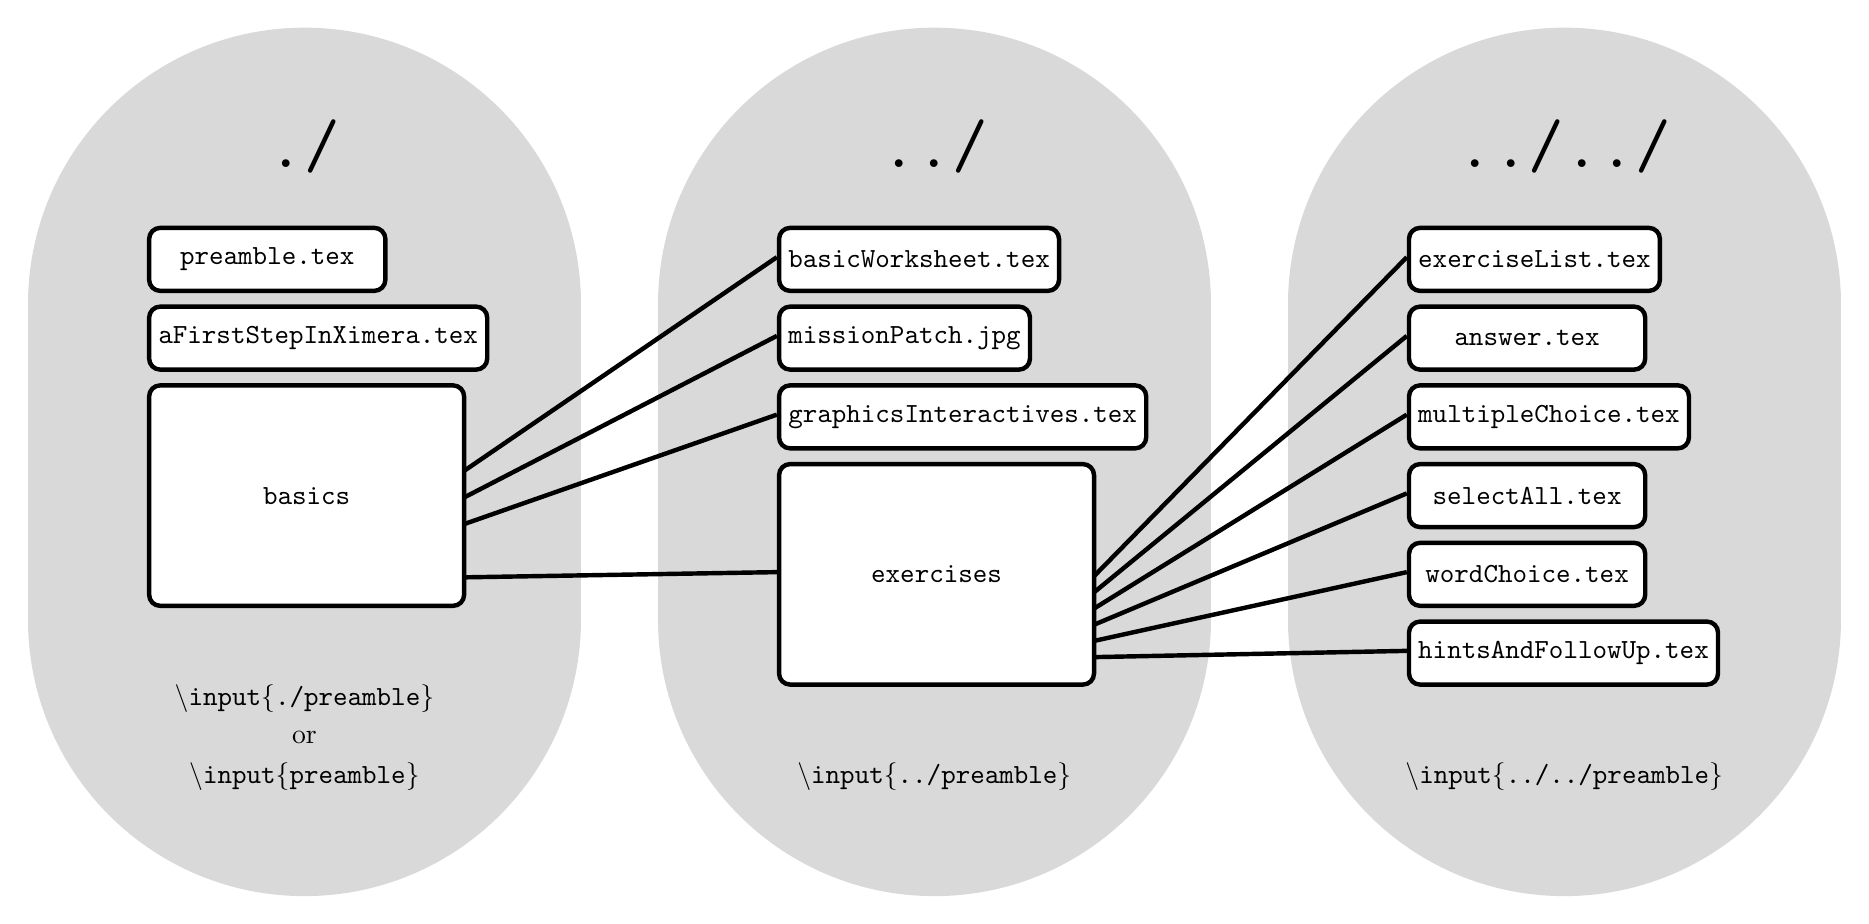
\begin{tikzpicture}
      % Define styles for nodes
      \tikzstyle{document} = [anchor=north west,draw, rounded corners,
      rectangle,
      minimum width=3cm,fill=white, minimum height=.8cm, ultra
      thick,font=\ttfamily]
      \tikzstyle{folder} = [anchor=north west,draw, rectangle, rounded corners,
      minimum width=4cm,fill=white, minimum height=2.8cm, ultra
      thick,font=\ttfamily]

      % Thick grey lines
      \draw[line width=200pt,white!85!black,line cap=round] (2,2) -- (2,-2);
      \draw[line width=200pt,white!85!black,line cap=round] (10,2) -- (10,-2);
      \draw[line width=200pt,white!85!black,line cap=round] (18,2) -- (18,-2);

      % Connections
      \draw[ultra thick] (2,-1.5) -- (8,2.6);
      \draw[ultra thick] (2,-1.5) -- (8,1.6);
      \draw[ultra thick] (2,-1.5) -- (8,.6);
      \draw[ultra thick] (2,-1.5) -- (8,-1.4);

      \draw[ultra thick] (11,-2.5) -- (16,2.6);
      \draw[ultra thick] (11,-2.5) -- (16,1.6);
      \draw[ultra thick] (11,-2.5) -- (16,.6);
      \draw[ultra thick] (11,-2.5) -- (16,-.4);
      \draw[ultra thick] (11,-2.5) -- (16,-1.4);
      \draw[ultra thick] (11,-2.5) -- (16,-2.4);

      % Symbols at top
      \node at (2,4) {\Huge \tt ./};
      \node at (10,4) {\Huge \tt ../};
      \node at (18,4) {\Huge \tt ../../};

      % Define the folders at top level
      \node[document] at (0,3) {preamble.tex};
      \node[document] at (0,2) {aFirstStepInXimera.tex};
      \node[folder] at (0,1) {basics};

      % Define the documents in the basics folder
      \node[document] at (8,3) {basicWorksheet.tex};
      \node[document] at (8,2) {missionPatch.jpg};
      \node[document] at (8,1) {graphicsInteractives.tex};
      \node[folder] at (8,0) {exercises};

      % Define the documents in the exercises folder
      \node[document] at (16,3) {exerciseList.tex};
      \node[document] at (16,2) {answer.tex};
      \node[document] at (16,1) {multipleChoice.tex};
      \node[document] at (16,0) {selectAll.tex};
      \node[document] at (16,-1) {wordChoice.tex};
      \node[document] at (16,-2) {hintsAndFollowUp.tex};

      % paths at bottom
      \node at (2,-3) {\tt\textbackslash input\{./preamble\}};
      \node at (2,-3.5) {or};
      \node at (2,-4) {\tt\textbackslash input\{preamble\}};
      \node at (10,-4) {\tt\textbackslash input\{../preamble\}};
      \node at (18,-4) {\tt\textbackslash input\{../../preamble\}};
    \end{tikzpicture}}
\end{center}
\twocolumn

\begin{verbatim}
%% where to find images
\graphicspath{  
{./}
{./graphicsVideosAndInteractives/}
}    
\end{verbatim}

\end{document}